\documentclass[a4paper,10pt]{article}

% Packages
\usepackage[utf8]{inputenc}
\usepackage{amsmath}
\usepackage{graphicx}
\usepackage{hyperref}
\usepackage{geometry}
\usepackage{parskip}
\usepackage{lmodern}
\usepackage{subcaption}
\usepackage{fullpage}

\usepackage{colortbl} % For coloring table cells and lines
\usepackage[table]{xcolor} % For more color options
\usepackage{booktabs}

\setlength{\parskip}{1em} % Adjust the length as needed

\geometry{a4paper, margin=0.8in}

% Title and Author
\title{Exercise 1: Classification}
\author{Florian Engl (12102619),\\ Lukas Sichert (12114770),\\ Kristof Dadic (12105475)}
\date{November 2024}

\begin{document}

% Title Page
\maketitle

% Table of Contents
%\tableofcontents


% Sections
\section{Datasets}

In this first chapter, we want to give a brief summary of the 4 datasets used in this exercise and discuss their most important characteristics.

\textbf{Congressional Voting:} This dataset contains 218 instances of 16 attributes in addition to the target attribute \emph{class}, which can take either the value \emph{democrat} or \emph{republican}. The distribution of these values is:
\begin{equation*}
    \text{democrat:}\,62\% \quad \text{republican:}\,38\%
\end{equation*}
All other attributes in the dataset represent significant issues on which members of the U.S. House of Representatives voted. Each instance in the dataset corresponds to the voting record of a single congressman on these 16 issues. The values of the attributes are \emph{y} if the congressman voted in favor of the issue, \emph{n} if the congressman voted against the issue, and \emph{unknown} if their position on the issue is not recorded. \\
The primary goal of the classification task is to predict a congressman’s political party affiliation based on their voting behavior. All attributes are categorical, taking only binary values. However, since some values are missing (marked as \emph{unknown}), data imputation will be required during preprocessing. Additionally, there is no need to scale the data because each attribute is already binary.

\textbf{Amazon Commerce Reviews:} This dataset contains 750 entries, each corresponding to a customer review sourced from Amazon. It includes 10,000 features along with a target variable labeled \emph{Class}. The target attribute consists of 50 distinct categories, each representing the first name of the reviewer. All other attributes correspond to individual English word, with integer values that indicate the frequency of each word’s occurrence in a review. \\
The objective is to determine the writer based on the frequency distribution of the words it contains. Given that the range of values for different features varies widely, scaling the data during preprocessing may improve performance. Notably, the dataset has no missing values.
\begin{figure}[h!]
    \centering
    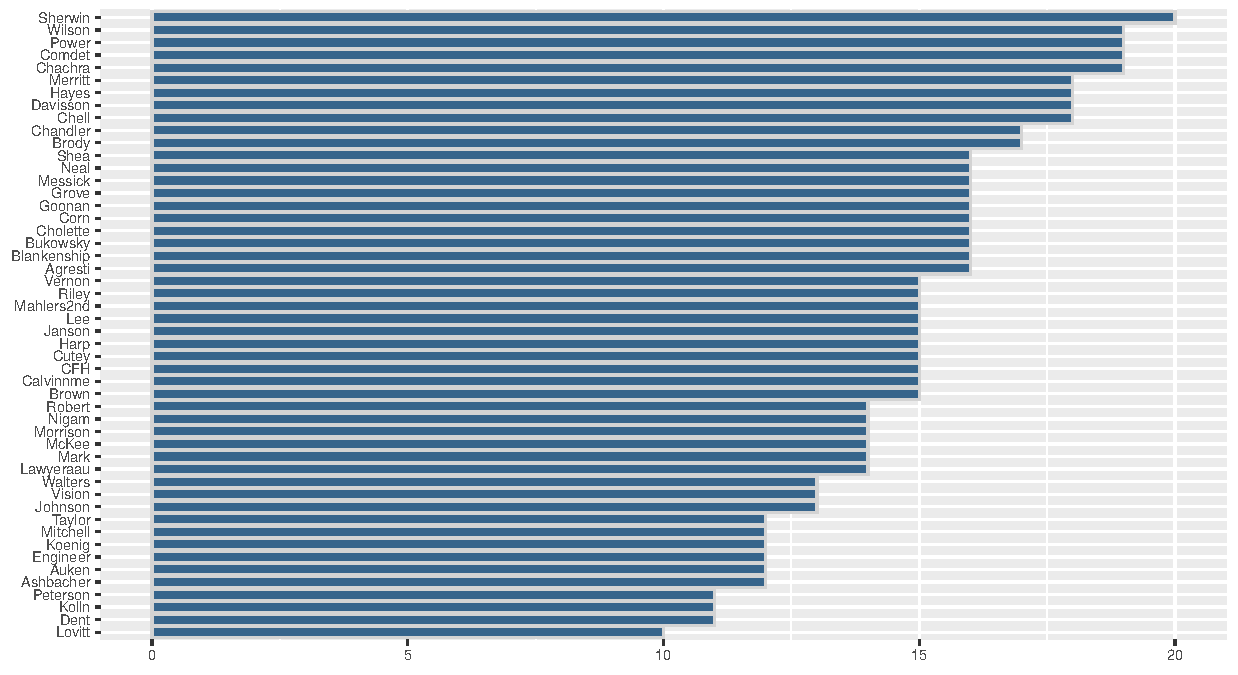
\includegraphics[width=0.75\linewidth]{amazon/plots/plot_amazon_classes.pdf}
    \caption{Distribution of target attribute for ”Amazon Commerce Reviews”}
    \label{fig:amazondist}
\end{figure}

\textbf{Census Income:} The "Census Income" dataset is derived from the 1994 U.S. Census database, maintained by the United States Census Bureau, a federal agency responsible for conducting the decennial U.S. census. The objective of this dataset is to predict whether an individual earns more than \$50,000 per year. The dataset contains 14 attributes plus the target variable, income, with 48,842 instances. The target variable is categorical, with two possible values $<=50K$ and $>50K$, distributed as follows:
\begin{equation*}
    <=\text{50K:}\,76\% \quad >\text{50K:}\,24\%
\end{equation*}        
Of the 14 attributes {age, fnlwgt, education-num, capital-gain, capital-loss,} and \emph{hours-per-week} are numerical and \emph{workclass, education, marital-status, occupation, relationship, race, sex,} and \emph{native-country} are categorical. Due to the varying ranges of the numerical features, scaling will likely be necessary during preprocessing. Additionally, the attributes workclass, occupation, and native-country contain missing values that must be handled as part of the data preparation process.

\textbf{Diabetes:} Finally, the "Diabetes" dataset contains medical records of Pima Indian women aged 21 and older, with all attributes related to diabetes. The objective is to build a machine learning model that predicts whether an individual has diabetes. The dataset includes 8 numerical features and a nominal target attribute, \emph{class}, with 768 instances. The target attribute is categorical, with two possible values \emph{tested\_negative} and \emph{tested\_positive} that are distributed as follows:
\begin{equation*}
    \text{tested\_negative:} \,65\% \quad \text{tested\_positive:}\,35\%
\end{equation*} 
Since the numerical attributes have significantly different ranges, scaling may be necessary during preprocessing to improve model performance.

\section{Classifiers}

Here, we want to provide insight into the classifiers we selected for our project and explain our reasoning behind these choices. We ultimately chose the random forest Classifier, the Linear Support Vector Classifier, and the ridge classifier, all implemented using the scikit-learn Python library.

First, we wanted to include at least one classifier from the lecture, as a practical application of the theoretical knowledge we gained during the lectures. Upon reviewing examples of how others approach classification tasks, it became evident that random forests are a very popular choice. When we tested this classifier on our initial dataset, "Congressional Voting," it delivered excellent results right away. Therefore, we decided to include random forests as the first classifier in our project. One major advantage of the random forest classifier is its inherent support for multi-class classification, which is particularly beneficial for datasets like "Amazon Commerce Reviews." Random forests are part of the ensemble methods family, which combines the predictions of multiple base estimators to reduce variance. Specifically, the employed algorithm constructs several decision trees and averages their predictions. This approach not only minimizes variance but also mitigates the overfitting tendencies of individual decision trees. However, one potential drawback is a slight increase in bias.

Selecting an appropriate classifier for the "Amazon Commerce Reviews" dataset posed some challenges due to its high dimensionality. Additionally, the dataset is sparse, with most attribute values being zero, and it contains a limited number of instances, providing only minimal information for each of the 50 classes. After researching potential solutions, we identified support vector machines (SVMs) as a suitable choice for high-dimensional, sparse data. Although SVMs are primarily designed for binary classification tasks, they can handle multi-class datasets using appropriate strategies. SVMs operate by constructing one or more hyperplanes to separate data points into distinct classes, aiming to maximize the margin (also called decision boundary) between the nearest data points of each class. If the data is not linearly separable, kernel methods can be employed to map the data into a higher-dimensional space where separation becomes feasible. \\
In scikit-learn, two SVM classifiers are available: the Linear Support Vector Classifier (LinearSVC) and the Support Vector Classifier (SVC). While SVC can use a linear kernel, it is not equivalent to LinearSVC due to differences in their underlying implementations. Additionally, LinearSVC is specifically recommended for large datasets. After testing both classifiers on our dataset, we concluded that in terms of accuracy, both options yield similar results when employing linear kernels, except on the "Amazon Commerce Reviews" Dataset, where LinearSVC fared better, but LinearSVC outperforms SVC in terms of runtime, which is why we chose this as our second classifier. For multi-class classification, LinearSVC employs the "one-vs-the-rest" strategy, training a separate model for each class in the target variable. Based on these results, we selected LinearSVC as our second classifier.

For the last classifier, we opted for a straightforward yet still quite effective approach. After exploring various classifiers available in scikit-learn, we decided to focus on linear models. Preliminary testing with our datasets revealed that the ridge classifier performed really well in terms of both efficiency and accuracy. Paired with the fact that one member of our team already has some theoretical knowledge in ridge regression due to his econometrics course, we decided to go with it for this project. 
In short, ridge regression is an enhanced version of linear regression that incorporates a penalty term into the cost function to reduce the risk of overfitting. This penalty term is regulated by a hyperparameter, which determines the degree of regularization. While a higher value can help mitigate overfitting, setting it too high may result in underfitting. This method is suitable for binary classification when the target variable is mapped to the values $\{-1, 1\}$. For multi-class classification, the ridge classifier uses multi-output regression, where multiple numerical outputs are predicted for each input.

\section{Evaluation}

When evaluating a classifier's performance on a dataset, several factors need to be considered. These include selecting appropriate performance metrics and determining how to split the data into training and testing sets. For our analysis, we employed repeated stratified k-fold cross-validation for each classifier and dataset. In this approach, the data is divided into k equally sized groups, or folds. At each step, k-1 folds are used for training, and the remaining fold is used for validation, resulting in the classifier being trained k times. The term stratified means that each fold maintains approximately the same class distribution as the original dataset, while repeated means that this process is performed multiple times. This method offers several advantages. By using multiple folds, the evaluation becomes less sensitive to the specific split of the data, as performance is averaged across k different splits. Repeating this process further reduces result variance. Stratified cross-validation is particularly beneficial for imbalanced datasets, as it guarantees that all training and test sets reflect the original class distribution. However, this method introduces the challenge of avoiding data leakage, which we address in the preprocessing section.

When choosing the number of folds and repetitions, a balance must be struck. Increasing repetitions improves result accuracy up to some point, but increases the runtime. Regarding the number of folds, small datasets or imbalanced classes may suffer if the test sets become too small or fail to represent all classes. In such cases, fewer folds are preferable. An alternative to cross-validation is the holdout method, where the dataset is split once into training and test sets. However, this method is less reliable unless the dataset is very large. We will revisit this in the Conclusion section.

Now focusing on the performance measures, we can differentiate between effectiveness and efficiency. Firstly, efficiency refers to the time required to train the model and classify new data. The importance of training time versus classification time depends on the use case. In most real-world scenarios, fast classification is prioritized, while training time is less critical since it is typically a one-time process.
For this project, though, we aimed to compare different preprocessing techniques and hyperparameters across three classifiers to identify the best-performing configurations. This required numerous evaluations using repeated stratified k-fold cross-validation, involving both training and testing. As a result, both training and classification times were important considerations, though training typically takes longer. To measure efficiency, we used the runtime for a single train-test split (using a 70\%-30\% holdout split). This approach allowed us to fairly compare classifiers across datasets, as the number of folds and repetitions varied between datasets and classifiers.

When evaluating effectiveness, several metrics can be used. The most commonly used is accuracy, which is calculated as the ratio of correct predictions to the total number of predictions. While accuracy provides a general sense of a classifier’s performance, it can be misleading for imbalanced datasets. For instance, if 99\% of the samples belong to one class and only 1\% to another, a simple dummy classifier that predicts the majority class for all samples would achieve 99\% accuracy. While this might seem like a good result, it is deceptive, as the classifier has not actually learned anything meaningful. Both the "Amazon Commerce Reviews" and "Census Income" datasets are moderately imbalanced. As a result, we decided to use accuracy as one of the evaluation metrics but remained cautious about its limitations in these cases. In addition to accuracy, precision and recall are also widely used metrics. Precision measures the proportion of all correct positive predictions. Thus, high precision indicates a low false positive rate. Recall measures the proportion of actual positives that were correctly identified. Thus, high recall minimizes false negatives. While both precision and recall are valuable, they are often inversely related. To balance these metrics, the F-score combines them into a single value. For all datasets expect "Diabetes", we chose the F1 score, defined as:
\begin{equation*}
    F1=\frac{2 \text{precision} \cdot \text{recall}}{\text{precision} + \text{recall}}
\end{equation*}
The closer the F1 score is to 1, the better the model's performance. However, a low F1 score can be less informative, as it might result from poor precision, poor recall, or both. One of the strengths of precision, recall, and F1 scores is their suitability for evaluating models on imbalanced datasets. For this reason, we chose the F1 score as the primary metric for three out of the four datasets. The exception was the "Diabetes" dataset, where we prioritized recall instead. In this case, the primary objective is to minimize false negatives, as misclassifying a sick person as healthy could have serious consequences. Conversely, false positives are less concerning, as individuals flagged as potentially positive are likely to undergo further medical testing for confirmation. We summarized the effectiveness measures for each dataset in the table below.

\begin{table}[h]
\centering
\begin{tabular}{|c|c|c|}
\hline
Dataset & Measure 1 & Measure 2 \\ \hline
Congressional Voting & Accuracy & F1 Score \\ 
Amazon Commerce Reviews & Accuracy & F1 Score (macro) \\ 
Census Income & Accuracy & F1 Score \\ 
Diabetes & Accuracy & Recall \\ \hline
\end{tabular}
\caption{Effectiveness measures}
\label{tab:effectiveness_measures}
\end{table}
In the brief explanation of the F1 score above, we focused on binary data. However, the "Amazon Commerce Reviews" dataset is multi-class. In scikit-learn, there are three methods for calculating the F1 score for multi-class data, controlled by the average parameter: 'micro', 'macro', and 'weighted'. For this project, we chose the 'macro' approach. In this method, the F1 score is computed separately for each class in a "one-vs-the-rest" fashion and then averaged across all classes. This ensures that each class contributes equally to the final score, regardless of its frequency in the dataset. In contrast, the 'weighted' approach accounts for class imbalance by weighting each class's F1 score proportionally to its representation in the data and the 'micro' approach counts the global true positives, false positives and false negatives and directly computes the F1 score, therefore giving each instance the same weight regardless of class.  We compared all variants in preliminary tests across all datasets we use the F1 score in, since they are also applicable in the binary case, and chose to go with the "regular" F1-score for the datasets "Congressional Voting" and "Census Income" and the 'macro' F1-Score for "Amazon Commerce Reviews".

Despite careful consideration in selecting performance metrics, they are not "sufficient" to guarantee that the trained model will perform equally well on unseen data. Metrics can only guide us in evaluating a model's performance based on the available data and its intended use case.

\section{Preprocessing}
\label{sec:preprocessing}
We will do four different measures to properly preprocess the data. These are: data imputation, encoding of categorical variables,
scaling of numerical values and dimensionality reduction. In this section we will look at each dataset and 
describe which tasks can be used on the dataset and how a specific task is performed. Then we will compare the different
settings for all the models and determine their effectiveness using measures described in the previous section. 
In order to make this a meaningful comparison, we will use the default hyperparameters for all classifiers and 
we will split the data equally in the cross-validation.

One thing we have to be careful with is Data leakage. Data leakage occurs when data is preprocessed before it was split into the training and test set. This way information 
from the test set is used to preprocess the training set. For example the MinMaxScaler uses the minimum and maximum values 
to scale these values properly. The values should only be computed on the training set and then be used on both training and 
test set. This can get rather difficult when using cross-validation. In order to avoid this, we will use pipelines.    
Pipelines are a feature of scikit-learn that allow the chaining of multiple transformers and estimators and also avoid 
data leakage. We will define a different pipeline for each preprocessing task and variant and chain these pipelines to compare 
the different settings.

\textbf{Congressional Voting:} As this dataset contains missing values we will need a strategy to impute these values. 
It is important to note that the missing values are all labeled as \textit{'unknown'}.
As all the values are categorical there are two possible strategies for data imputation.
We can either use the most frequent value of the respective attribute in the training dataset
or we can treat the missing values as a separate category. We will use one-hot-encoding for the categorical values,
except for the binary ones. Binary values will be encoded as 0 and 1. By using one-hot-encoding
the two different treatments of the missing values will yield a different encoding. Still all the values remain binary, 
so no further scaling is needed. As the dataset is rather small, we will not use dimensionality reduction. This means
that we will only compare the two different strategies for data imputation.
In table~\ref{table:imputation} the results are visualized for the different classifiers.
Here the right number in each cell is the average accuracy and the left number is the average F1 score.

\begin{table}[h!]
\centering
\begin{tabular}{|c|c|c|c|}
\hline
\textbf{Data Imputation} & \textbf{Random Forest} & \textbf{LinearSVC} & \textbf{Ridge} \\
\hline
\textsf{most frequent} & \cellcolor[HTML]{C1E1C1}0.957/0.949 & \cellcolor[HTML]{C1E1C1}0.962/0.954 & \cellcolor[HTML]{C1E1C1}0.963/0.957 \\
\hline
\textsf{nan is category} & 0.955/0.947 & 0.955/0.947 & 0.960/0.953 \\
\hline
\end{tabular}
\caption{Comparison of data imputation for different classifiers for "Congressional Voting" dataset}
\label{table:imputation}
\end{table}
For every classifier the most frequent value imputation strategy yields better results for both accuracy and F1 score.
In this test we used 5 folds and 10 repetitions for the cross-validation.

\textbf{Amazon Commerce Reviews:} This dataset contains no missing values, therefore we don't need to impute any values.
The target attribute has 50 different values, which will be encoded as \textit{0,1,2\ldots,49}. 
All the other values are numerical, therefore we will try different scaling strategies.
We will try the most common scalers in the scikit-learn library, namely 
\begin{itemize}
    \item the MinMaxScaler which scales each feature to a given range, which is by default 0 to 1,
    \item the MaxAbsScaler which divides each feature by the maximum absolute values of the respective attribute,
    \item the StandardScaler which divides each feature by the standard deviation of the attribute,
    \item the RobustScaler which subtracts the median from each value and divides the result by the interquartile range of the respective attribute,
    \item the PowerTransformer which applies a power transformation to make the data more Gaussian-like,
    \item the QuantileTransformer which transforms the data to follow a uniform distribution.
\end{itemize}
The Transformers and the RobustScaler are known to be robust to outliers. We have also tested a method for dimensionality reduction called
principal component analysis (PCA). This method is used to reduce the number of features by projecting the data onto a lower dimensional space. 
The n\_components= 0.95 parameter determines, that our data should be projected onto the number of dimensions that explain 95\% of the variance.
Again the results are visualized in table~\ref{table:scaling}.

\begin{table}[h!]
\centering
\small
\begin{tabular}{|c|c|c|c|c|}
\hline
\textbf{Scaler} & \textbf{Dim Reduction} & \textbf{Random Forest} & \textbf{LinearSVC} & \textbf{Ridge} \\
\hline
StandardScaler & none & 0.577/0.537 & 0.717/0.689 & 0.692/0.669 \\
\hline
MaxAbsScaler & none & 0.577/0.536 & 0.732/0.707 & 0.699/0.680 \\
\hline
None & none & 0.578/0.537 & 0.613/0.582 & 0.580/0.549 \\
\hline
MinMaxScaler & none & 0.577/0.536 & 0.640/0.622 & 0.649/0.631 \\
\hline
RobustScaler & none & 0.576/0.535 & 0.672/0.641 & 0.595/0.567 \\
\hline
QuantileTransformer & none &  0.581/0.543 & 0.739/0.712 & 0.696/0.671 \\
\hline
PowerTransformer & none &   \cellcolor[HTML]{C1E1C1} 0.581/0.544 & \cellcolor[HTML]{C1E1C1}  0.742/0.714 & 0.733/0.710 \\
\hline
MaxAbsScaler & pca & 0.225/0.198 & 0.670/0.647 & 0.730/0.706 \\
\hline
RobustScaler & pca & 0.266/0.228 & 0.528/0.500 & 0.637/0.603 \\
\hline
None & pca & 0.257/0.220 & 0.466/0.434 & 0.622/0.581 \\
\hline
StandardScaler & pca & 0.257/0.237 & 0.604/0.580 & 0.725/0.697 \\
\hline
MinMaxScaler & pca & 0.233/0.206 & 0.573/0.557 & 0.621/0.610 \\
\hline
QuantileTransformer & pca & 0.229/0.198 & 0.663/0.637 & 0.715/0.687 \\
\hline
PowerTransformer & pca & 0.231/0.214 & 0.677/0.647 & \cellcolor[HTML]{C1E1C1}  0.754/0.729 \\
\hline
\end{tabular}
\caption{Comparison of different numeric scalers and dimensionality reduction techniques for the "Amazon Commerce Reviews" dataset}
\label{table:scaling}
\end{table}







In the above Experiment we have used 5 folds and 10 repetitions for the cross-validation. The best results are achieved by the PowerTransformer for all classifiers. However, only the ridge classifier benefited from the
dimension reduction.


\textbf{Census Income:} This dataset has missing values, but only for categorical values.
 Those values are labeled with \textit{'?'}. We will try the same two strategies as for the "Congressional Voting" dataset.
 The only exception is the \textit{'education'} column. This column is already encoded as the
 \textit{'education-num'} column and will therefore be dropped. For the numeric columns 
 we tested the same numerical scalers, which we tried for the 
 "Amazon Commerce Reviews" dataset. Since the dataset only has 14 features,
we will not use dimensionality reduction. Like for the previous
datasets we will present the result in a table, where the first score in each cell is accuracy and the second
number is the F1 score.

\begin{table}[h!]
\centering
\small
\begin{tabular}{|c|c|c|c|c|}
\hline
\textbf{Scaler} & \textsf{Data Imputation} & \textbf{Random Forest} & \textbf{LinearSVC} & \textbf{Ridge} \\
\hline
StandardScaler & most frequent & \cellcolor[HTML]{C1E1C1}0.857/0.677 & 0.852/0.655 & 0.841/0.607 \\
\hline
MaxAbsScaler & most frequent & 0.857/0.676 & 0.851/0.654 & 0.841/0.607 \\
\hline
None & most frequent & 0.857/0.676 & 0.800/0.379 & 0.830/0.567 \\
\hline
MinMaxScaler & most frequent & 0.857/0.676 & 0.852/0.654 & 0.841/0.607 \\
\hline
RobustScaler & most frequent & 0.857/0.676 & 0.851/0.649 & 0.830/0.561 \\
\hline
QuantileTransformer & most frequent & 0.857/0.676 & 0.845/0.645 & 0.842/0.621 \\
\hline
PowerTransformer & most frequent & 0.852/0.665 & 0.845/0.645 & 0.842/0.621 \\
\hline
MaxAbsScaler & \textit{'?'} is category & 0.857/0.676 & 0.853/0.659 & 0.841/0.610 \\
\hline
RobustScaler & \textit{'?'} is category & 0.857/0.676 & 0.852/0.658 & 0.841/0.610 \\
\hline
None & \textit{'?'} is category & 0.857/0.676 & 0.800/0.379 & 0.830/0.568 \\
\hline
StandardScaler & \textit{'?'} is category & 0.857/0.676 & \cellcolor[HTML]{C1E1C1}0.853/0.659 & 0.841/0.610 \\
\hline
MinMaxScaler & \textit{'?'} is category & 0.857/0.676 & 0.853/0.658 & 0.841/0.610 \\
\hline
QuantileTransformer & \textit{'?'} is category & 0.857/0.676 & 0.847/0.649 & \cellcolor[HTML]{C1E1C1}0.844/0.627 \\
\hline
PowerTransformer & \textit{'?'} is category & 0.852/0.666 & 0.846/0.645 & 0.843/0.623 \\
\hline
\end{tabular}
\caption{Comparison of different numeric and categorical transformers for the "Census Income" dataset}
\label{table:censustransformers}
\end{table}
We used 5 folds and 5 repetitions in the cross-validation for this experiment, except for the random forest
classifier. The random forest classifier was too slow, and we had to reduce the number of repetitions to 1.
For this dataset the best
preprocessing strategy was different for every classifier. The respective cells are marked in green in the
table above. After these experiments we decided to use the StandardScaler combined with setting missing
values as the most frequent category for the random forest classifier, the StandardScaler but with setting
missing values as an extra category for the linear support vector classifier and the QuantileTransformer
combined with setting missing values as an extra category for the ridge classifier.

\textbf{Diabetes:} This dataset does not have any missing values except for the target attribute. Therefore, we 
 don't need to consider data imputation. As the dataset is very low dimensional, we will not use any dimensionality reduction. 
 So we will only compare different scaling methods. We have used the already introduced scaling methods 
 and got the result shown in table~\ref{table:diabetesscalers}.
 \begin{table}[h!]
\centering
\begin{tabular}{|c|c|c|c|}
\hline
\textbf{Scaler} & \textbf{Random Forest } & \textbf{LinearSVC } & \textbf{Ridge } \\
\hline
MinMaxScaler & \cellcolor[HTML]{C1E1C1}0.767/0.592 & 0.770/0.553 & 0.768/0.542 \\
\hline
MaxAbsScaler & 0.767/0.590 & 0.771/0.553 & 0.769/0.543 \\
\hline
RobustScaler & 0.766/0.589 & 0.770/0.560 & 0.770/0.555 \\
\hline
None & 0.766/0.588 & \cellcolor[HTML]{C1E1C1}0.771/0.559 & 0.770/0.555 \\
\hline
StandardScaler & 0.766/0.589 & 0.770/0.560 & \cellcolor[HTML]{C1E1C1}0.770/0.555 \\
\hline
PowerTransformer & 0.766/0.592 & 0.763/0.564 & 0.761/0.554 \\
\hline
QuantileTransformer & 0.766/0.592 & 0.763/0.564 & 0.761/0.554 \\
\hline
\end{tabular}
\caption{Comparison of different scalers for the Diabetes dataset}
\label{table:diabetesscalers}
\end{table}
In the end we decided to use the scalers marked in green for the respective classifiers.\\







\section{Hyperparameters}
\label{sec:hyperparameters}
Now we want to take a closer look at the hyperparameters of our models. In a first step we want to optimize the hyperparameters for the different models and datasets.
In a second step we will analyze how sensitive the models are to changes in the hyperparameters. Unfortunately we will not be able to find the optimum for all hyperparameters, as scikit-learn offers a wide range, so we are going to focus on the most important ones.

For tuning we want to use Bayesian Optimization from the scikit-optimize package. Bayesian Optimization is a probabilistic approach to finding the minimum or maximum. This means that it builds a probabilistic model of the function and uses this model to decide on where to evaluate in the next step. In our case the function is given by the performance measure. 

Bayesian Optimization does not only take a function as input but a search space as well, which is why we need to decide on an appropriate range of values for the parameters as well. Moreover, because we chose two different performance measures for each dataset, we will have to do the optimization twice and then compare results to get the overall best.

\textbf{Random Forest Classifier:} The random forest classifier has a lot of hyperparameters and takes a comparatively long time to train and evaluate. That being the case we decided to focus the following five parameters to keep tuning times at a reasonable level. These are:

\begin{itemize}
    \item \textsf{n\_estimators}: This determines the number of trees in the forest.
\item \textsf{max\_depth}: This gives a maximum on the depth of the trees. If we set this to None, the trees will expand fully until each leaf has less than \textsf{min\_samples\_split} instances.
\item \textsf{min\_samples\_split}: Is the minimum number of instances necessary for an inner node to split.
\item \textsf{min\_samples\_leaf}: Is the minimum number of instances necessary for a leaf node. This means a split will only happen if both leaf nodes have at least \textsf{min\_samples\_leaf} instances afterwards.
\item \textsf{max\_features}: This gives the number of features that are being randomly selected from all features at each node to decide on the best split. Possible values are integers or floats and 'sqrt', 'log2', 'None' or 'auto'.
\end{itemize}


For the big datasets "Amazon Commerce Reviews" and "Diabetes" we will use the search space:
 

\begin{center}
    \parbox{0.75\textwidth}{%
    \raggedright
    \textsf{n\_estimators} \(\in\) \{100,\dots, 2000\}, \textsf{max\_depth} \(\in\) \{None, 10 \dots , 100\}, \\
    \textsf{min\_samples\_split} \(\in\) \{2, \dots, 100\}, \textsf{min\_samples\_leaf} \(\in\) \{1, \dots, 5\}, \\
    \textsf{max\_features} \(\in\) \{'sqrt', 'log2'\}.}
\end{center}

Here we didn't consider 'None' as a value for \textsf{max\_features} because it resulted in a runtime that was way too long for the scope of this project. Moreover, it is empirically known, that the other results usually give better values for classification. Nonetheless, on the other two datasets we could test \textsf{max\_features} = 'None' and could set the number of trees up to 3000, as these are significantly smaller datasets. For the other parameters we used the same search space as for the big datasets. In table \ref{table:tu_hyp_rf_ac} and \ref{table:tu_hyp_rf_f1} we summarized the results of our tuning process by giving the best values for the respective performance measures.

As already discussed we used the F1 score as a second metric for all datasets excepts the "Diabetes" dataset for which we used recall instead. It is also important to note that on the multiclass dataset "Amazon Commerce Reviews" we used the macro averaged F1 score and on the others the standard weighted one.

\begin{table}[h!]
    \centering
    \begin{tabular}{|c|c|c|c|c|c|c|}
    \hline
    Dataset & \textsf{estimators} & \textsf{depth} & \textsf{split} & \textsf{leafs} & \textsf{features} & accuracy \\
    \hline
    \multicolumn{7}{c}{\vspace{-0.4cm}} \\ % Adds vertical space
    \hline
    congressional voting & 1963 & 40 & 20 & 4 & None & 0.963 \\%20241111_151340
    \hline
    Amazon Reviews & 2000 & 50 & 2 & 1 & sqrt & 0.732 \\%new_tune_random_forest_20241117_133725
    \hline
    Census Income & 100 & 30 & 20 & 1 & sqrt & 0.865 \\%20241111_123502
    \hline
    diabetes & 3000 & 40 & 2 & 4 & sqrt & 0.773 \\%20241111_151657
    \hline
    \end{tabular}
    \caption{Tuned hyperparameters for random forest classifier and accuracy} 
    \label{table:tu_hyp_rf_ac}
    \end{table}

\begin{table}[h!]
    \centering
    \begin{tabular}{|c|c|c|c|c|c|c|}
    \hline
    Dataset & \textsf{estimators} & \textsf{depth} & \textsf{split} & \textsf{leafs} & \textsf{features} & F1/recall \\
    \hline
    \multicolumn{7}{c}{\vspace{-0.4cm}} \\ % Adds vertical space
    \hline
    congressional voting & 1963 & 40 & 20 & 4 & None & 0.957 \\%20241111_151340
    \hline
    Amazon Reviews & 2000 & 40 & 2 & 1 & sqrt & 0.704 \\%new_tune_random_forest_20241117_133725
    \hline
    Census Income & 2000 & 40 & 20 & 1 & sqrt & 0.686 \\%20241111_123502
    \hline
    Diabetes & 3000 & 70 & 6 & 4 & None & 0.623 \\%20241111_151657
    \hline
    \end{tabular}
    \caption{Tuned hyperparameters for random forest classifier and F1 score/recall} 
    \label{table:tu_hyp_rf_f1}
    \end{table}

We got the same results tuning for accuracy and for the F1 score on the first dataset. On the last three datasets we calculated the second performance measure with the best parameters for accuracy and got a F1 score of 0.698 for the "Amazon Commerce Review" dataset a F1 score of 0.685 for the "Census Income" dataset and a recall of 0.647 for the "Diabetes" dataset, so we will keep the parameter values for the best accuracy since they perform only slightly worse on the second performance measure than the optimal values.

\textbf{Linear Support Vector Classifier:} For support vector machines the arguably most important hyperparameter, apart from the type of kernel used, is the regularization parameter \textsf{C}. The Kernel in our case is always linear which leaves \textsf{C}. In addition we considered three other parameters, we thought to be interesting. The considered hyperparameters are:

\begin{itemize}
    \item \textsf{C}: The so-called regularization parameter. Its inverse is the strength of the regularization, which is why it has to be greater than 0. A strong regularization means a big loss if the decision boundary small.
\item \textsf{fit\_intercept}: It can be set to 'True' or 'False'. If set to 'True' the model will calculate the intercept for the decision boundary.
\item\textsf{class\_weight}: This parameter decides how much the model should take into account classifying differently sized classes. In unbalanced datasets for example it can be useful to give a bigger weight to correctly classifying the minority class in order to prevent the model overly predicting the majority class. We only considered the values 'balanced' and 'None' but you could assign specific weights for each class. When set to 'balanced' the weights are inversely proportional to class sizes.
\item \textsf{dual}: Takes the values 'True' or 'False' and decides whether the primal or the dual problem is solved. Generally the dual Problem is faster especially for high dimensional data, but as we will see sometimes you get better results with the primal problem.
\end{itemize}

As already discussed, the influence of the \textsf{class\_weight} will be especially interesting for our imbalanced datasets. For the linear support vector classifier we used the following search space on all four datasets:

\begin{center}
    \parbox{0.55\textwidth}{%
    \raggedright
    \textsf{C}\(\in[10^{-6},10^{6}]\), \textsf{fit\_intercept}\(\in\){True,False},\\ \textsf{class\_weight}\(\in\){'balanced','None'}, \textsf{dual}\(\in\){True,False}.	
    }
\end{center}

Again we summarized the results of our optimization process in table \ref{table:tu_hyp_svc_ac} and \ref{table:tu_hyp_svc_f1}.

\begin{table}[h!]
    \centering
    \begin{tabular}{|c|c|c|c|c|c|}
    \hline
    Dataset & \textsf{C} & \textsf{fit\_intercept} &  \textsf{class\_weight} & \textsf{dual} & accuracy \\
    \hline
    \multicolumn{6}{c}{\vspace{-0.4cm}} \\ % Adds vertical space
    \hline
    congressional voting & 1.150 & True & balanced & False & 0.963 \\%20241111_151511
    \hline
    Amazon Reviews & 0.00266 & True & balanced & False & 0.751 \\%new20241119_1101235
    \hline
    Census Income & 679.520 & True & None & False & 0.853 \\%20241111_093143
    \hline
    diabetes & 2.353 & True & None & False  & 0.771 \\%20241111_150042
    \hline
    \end{tabular}
    \caption{Tuned hyperparameters for linear support vector classifier and accuracy} 
    \label{table:tu_hyp_svc_ac}
    \end{table}

\begin{table}[h!]
    \centering
    \begin{tabular}{|c|c|c|c|c|c|}
    \hline
    Dataset & \textsf{C} & \textsf{fit\_intercept} &  \textsf{class\_weight} & \textsf{dual} & F1/recall \\
    \hline
    \multicolumn{6}{c}{\vspace{-0.4cm}} \\ % Adds vertical space
    \hline
    congressional voting & 1.241 & True & None & False & 0.955 \\%20241111_151511
    \hline
    Amazon Reviews & 0.00350 & True & balanced & False &  0.729 \\%new20241119_101235
    \hline
    Census Income & 0.274 & True & balanced & False & 0.677 \\%20241111_093143
    \hline
    Diabetes & 1e-06 & False & balanced & False  & 0.838 \\%20241111_150042
    \hline
    \end{tabular}
    \caption{Tuned hyperparameters for linear support vector classifier and F1 score/recall} 
    \label{table:tu_hyp_svc_f1}
    \end{table}
    
The results show, that the computation with the primal problem outperformed the dual problem in every case. However, it should be noted that for the "Amazon Commerce Reviews" dataset we got the same accuracy and F1 score for dual computation. Therefore, we will choose the dual computation as it is faster.

Later we will see that small changes in \textsf{C} do not vary the result too much, so we choose \textsf{C}=0.003 for "Amazon Commerce Reviews" and \textsf{C} =1.2 for "Congressional Voting". Taking the other values from table \ref{table:tu_hyp_svc_ac} for "Congressional Voting" we get an F1 score of 0.951 which is pretty good, so we will use these values.

For the other two datasets finding the right values for optimizing both performance measures at the same time is harder because they differ quite a lot. The "Census Income" dataset is imbalanced, which is why we would usually prefer the values in table \ref{table:tu_hyp_svc_f1}. This gives us an accuracy of 0.805. But using the values from table \ref{table:tu_hyp_svc_ac} the F1 score is 0.659312, which is less of a difference to the optimal value than our loss in accuracy would be otherwise, so we choose these values.

To the "Diabetes" dataset we will get back later in the sensitivity analysis because, as we will see, matters are more complicated for this dataset.

\textbf{Ridge Classifier:}
As for the linear support vector classifier the arguably most influential parameter is the regularization parameter called \textsf{alpha}. For the ridge classifier the regularization punishes high weights which again helps to prevent overfitting. \textsf{alpha} for the ridge classifier correspond to the value \(\frac{1}{2 \text{\textsf{C}}}\) and therefore has to be positive.\\
We also considered two other parameters, which we already encountered when tuning the linear support vector classifier, namely \textsf{fit\_intercept} and \textsf{class\_weight}. The search space we considered is:
\begin{center}
    \textsf{alpha}\(\in[0,100]\), \textsf{fit\_intercept}\(\in\){True,False}, \textsf{class\_weight}\(\in\){'balanced','None'}.
\end{center}

Once more table \ref{table:tu_hyp_ridge_ac} shows the tuned parameters for the accuracy and table \ref{table:tu_hyp_ridge_f1} for the F1 score/recall.

\begin{table}[h!]
    \centering
    \begin{tabular}{|c|c|c|c|c|}
    \hline
    Dataset & \textsf{alpha} & \textsf{fit\_intercept} &  \textsf{class\_weight} &  accuracy \\
    \hline
    \multicolumn{5}{c}{\vspace{-0.4cm}} \\ % Adds vertical space
    \hline
    congressional voting & 0 & True & None & 0.963 \\%20241111_122418
    \hline
    Amazon Reviews & 45.32 & False & None &  0.754 \\%20241111_110048
    \hline
    Census Income & 63.876 & True & None &  0.844 \\%20241111_121945
    \hline
    Diabetes & 0 & True & None &  0.771 \\%20241111_151531
    \hline
    \end{tabular}
    \caption{Tuned hyperparameters for ridge classifier and accuracy} 
    \label{table:tu_hyp_ridge_ac}
    \end{table}

\begin{table}[h!]
    \centering
    \begin{tabular}{|c|c|c|c|c|}
    \hline
    Dataset & \textsf{alpha} & \textsf{fit\_intercept} &  \textsf{class\_weight} & F1/recall \\
    \hline
    \multicolumn{5}{c}{\vspace{-0.4cm}} \\ % Adds vertical space
    \hline
    Congressional Voting & 0 & True & None & 0.963 \\%20241111_122418
    \hline
    Amazon Reviews & 45.32 & False & None &  0.730 \\%20241111_110048
    \hline
    Census Income & 11.333 & True & balanced & 0.666 \\%20241111_121945
    \hline
    Diabetes & 0 & False & balanced & 0.797 \\%20241111_11531
    \hline
    \end{tabular}
    \caption{Tuned hyperparameters for ridge classifier and F1 score/recall} 
    \label{table:tu_hyp_ridge_f1}
    \end{table}

For "Congressional Voting" and "Amazon Commerce Reviews" the values in table \ref{table:tu_hyp_ridge_ac} and table \ref{table:tu_hyp_svc_f1} coincide, so those are the best settings. 

For the "Census Income" dataset testing the values for the best accuracy gave us a F1 score of 0.626 and vice versa we got an accuracy of 0.795. In this case the loss in accuracy is comparable to the loss in the F1 score, so we choose the values from table \ref{table:tu_hyp_ridge_f1}. Doing this we take into account that the dataset is imbalanced and prevent the model from exploiting the different class sizes.

Again we will revisit the "Diabetes" dataset later in the sensitivity analysis to analyze the best parameter setting for overall performance.


For the tuning and testing processes, we always used repeated stratified 5-fold crossvalidation. On the "Congressional Voting" and the "Diabetes" dataset we used 10 repetitions and on the other two datasets we used 5 repetitions except for the random forest classifier with which we did only one repetition. This was due to the otherwise very long runtime for the large datasets.

The next step in analyzing the influence of hyperparameters on our classifiers is the sensitivity analysis. This means we will take a look at how changing a single parameter value influences the performance of the model. We will do this for the hyperparameters we tuned in the previous section and will always change one while keeping the others at their optimal values, which we found earlier. We are going to achieve this by plotting the effectiveness measures against the parameter values.\\
However, for the "Diabetes" Dataset in combination with the linear support vector classifier and the ridge classifier we will take a closer look and try all combinations of \textsf{fit\_intercept} and \textsf{class\_weight} and vary the parameters \textsf{C} and \textsf{alpha} because we still need to decide on the overall best setting.

\textbf{Random Forest Classifier Sensitivity:}
We first want to find out how much each of the 5 considered hyperparameters influences the effectiveness of the classifier. We found that the sensitivity highly depends on the dataset:

\begin{itemize}
    \item \textsf{n\_estimators}: On the datasets "Census Income" and "Diabetes", the parameter changed almost nothing. However, for 'Amazon Commerce Reviews we got a clear Trend, that both measures increased with the number of trees first rather quickly and then more slowly. For the "Congressional Voting" dataset the parameter seemed to influence the effectiveness but we no clear trend could be identified. 
\item \textsf{max\_depth}: Varying this parameter only changed the effectiveness for the "Amazon Commerce Reviews"  and the "Census Income" dataset. Here we could see that the accuracy increased with the depth of the trees at first and then stagnated, but the increase in accuracy for "Census Income" was almost negligible and the increase in the F1 score was also way smaller than for "Amazon Commerce Reviews".

\item \textsf{min\_samples\_split}: For the "Census Income" and the "Diabetes" datasets varying this parameter hardly changed the effectiveness scores. On "Amazon Commerce Reviews" both scores decreased with higher values whereas for the "Congressional Voting" dataset both values decreased to a minimum at \\ \textsf{min\_samples\_split}=5 and then increased to the original value again.
\item \textsf{min\_samples\_leaf}: This parameter did not really influence the performance for the "Diabetes" and "Census Income" datasets. For the other two, small values fared better which fits in with our optimized values.
\item \textsf{max\_features}: 'sqrt' consistently outperformed 'log2' by quite a big margin on the "Amazon Commerce Reviews" dataset. For the "Census Income" it does not make much of a difference. On our smaller and less dimensional datasets 'None' led to the best results except for the accuracy of "Diabetes" where 'sqrt' performed a little better.
\end{itemize}

To underline our conclusions we want to give a few exemplary plots in figure \ref{fig: sensitivity rf} below. 

\begin{figure}[h!]
    \captionsetup{justification=centering}
    \begin{subfigure}[b]{0.45\textwidth}
        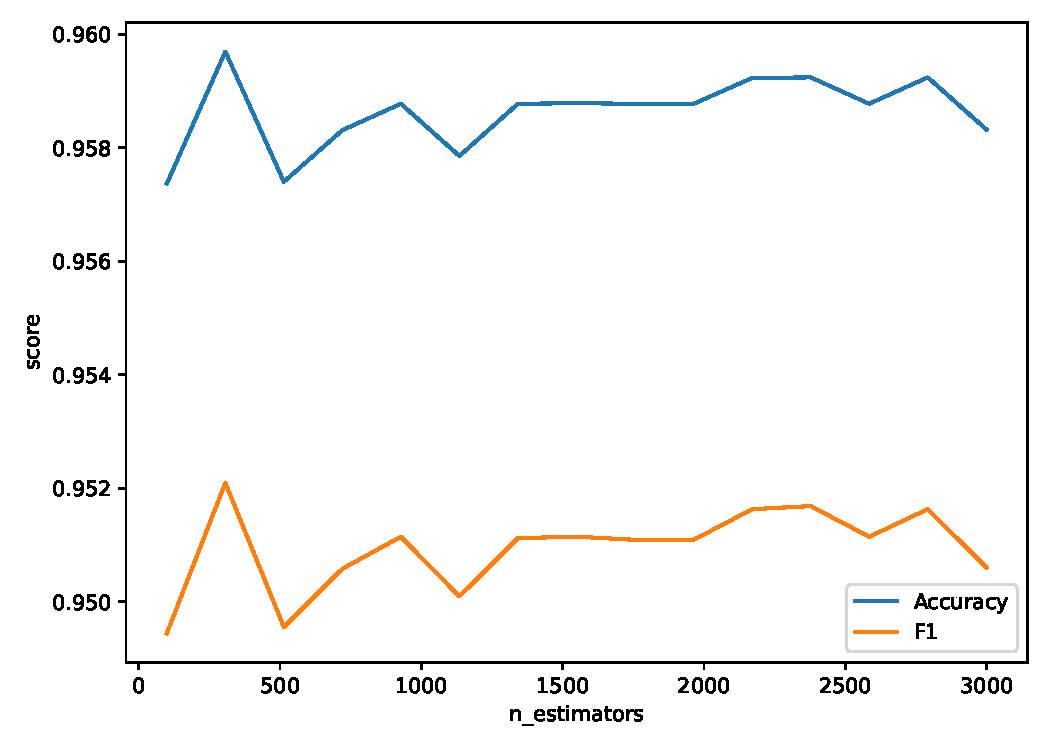
\includegraphics[width=\textwidth]{congress/plots/RandomForestClassifier_n_estimators_sensitivity.pdf}
        \caption{Parameter \textsf{n\_estimators} for dataset "Congressional Voting"}
    \end{subfigure}
    \hfill
    \begin{subfigure}[b]{0.45\textwidth}
        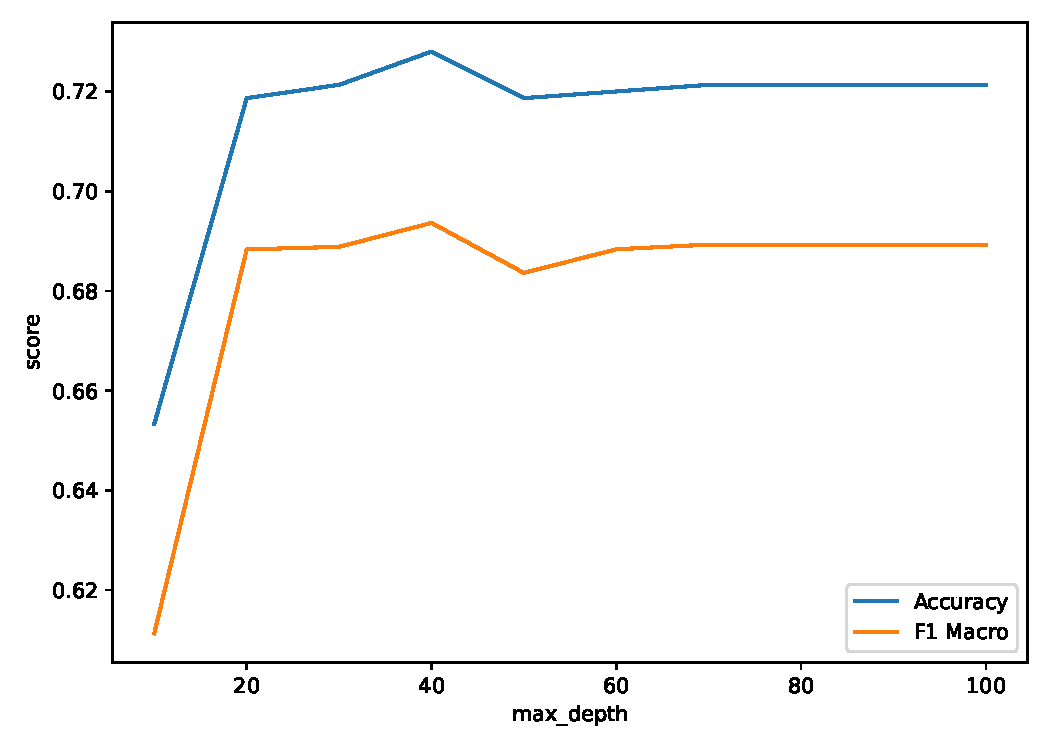
\includegraphics[width=\textwidth]{amazon/plots/RandomForestClassifier_max_depth_sensitivity.pdf}
        \caption{Parameter \textsf{max\_depth} for dataset "Amazon Commerce Reviews"}
    \end{subfigure}
    \vfill
    \begin{subfigure}[b]{0.45\textwidth}
        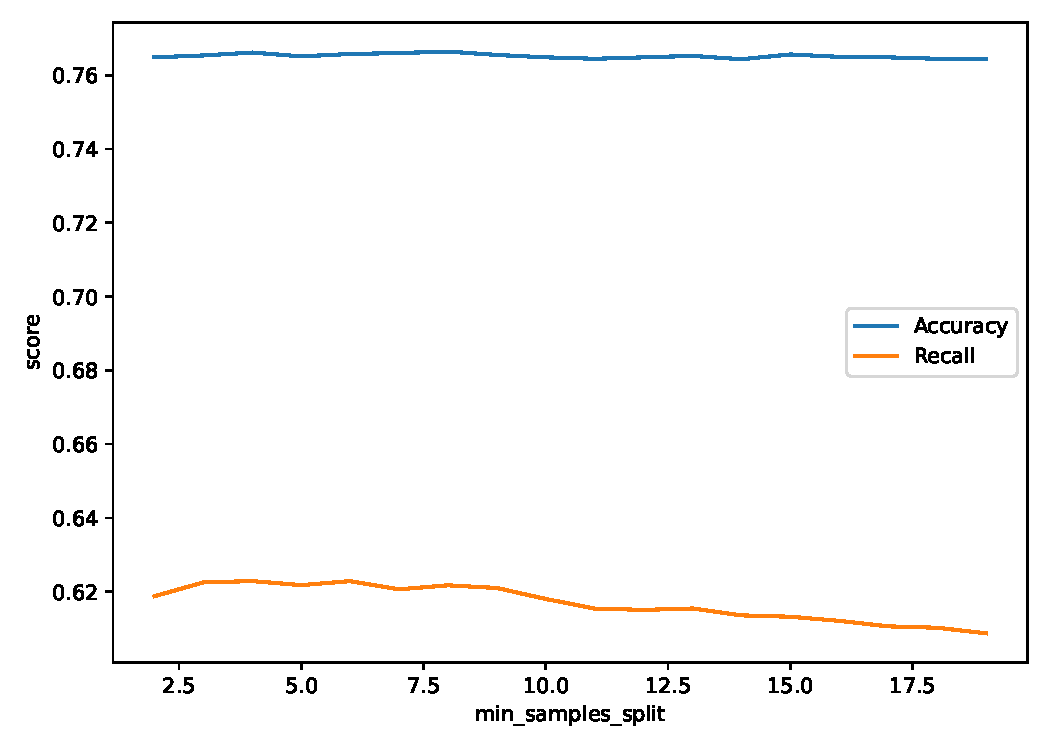
\includegraphics[width=\textwidth]{diabetes/plots/rf_min_samples_split_sensitivity.pdf}
        \caption{Parameter \textsf{min\_samples\_split} for dataset "Diabetes"}
    \end{subfigure}
    \hfill
    \begin{subfigure}[b]{0.45\textwidth}
        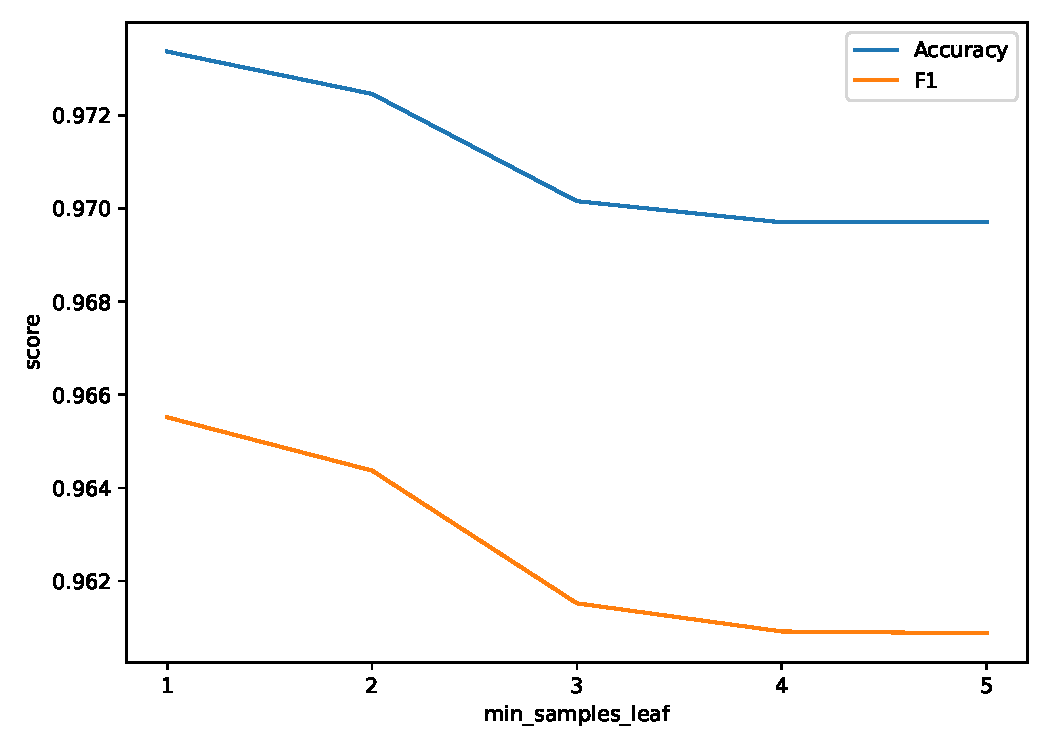
\includegraphics[width=\textwidth]{congress/plots/RandomForestClassifier_min_samples_leaf_sensitivity.pdf}
        \caption{Parameter \textsf{min\_samples\_leaf} for dataset "Congressional Voting"}
    \end{subfigure}
    \caption{Sensitivity analysis of random forest classifier}
    \label{fig: sensitivity rf}
\end{figure}


\textbf{Linear Support Vector Classifier Sensitivity:}

The parameter \textsf{C} had significant influence on the performance for every dataset except the "Census Income" one, where only the F1 score increased at first and then also stagnated.\\
Setting \textsf{class\_weight} to 'balanced' improved the F1 score/recall for every dataset as expected but also improved the accuracy for the "Amazon Commerce Reviews" and the "Congressional Voting" dataset. On the other datasets it decreased the accuracy, so there is no overall conclusion as to what setting to use as it depends not only on the dataset but also on the preferred performance measure.\\
For the parameter \textsf{fit\_intercept}, we found that setting the intercept to 'True' yielded the best results for accuracy and F1 score across all datasets. When considering the recall on the "Diabetes" dataset, \textsf{fit\_intercept}=False performed slightly better, but the overall best choice was again False, as we will see later.\\
The parameter \textsf{dual} gave better results for accuracy and recall when set to 'False' for the "Census Income" dataset. On the other datasets it did not make much of a difference, only the accuracy on the "Diabetes" dataset was slightly better when setting \textsf{dual} to 'False'.

\begin{figure}[h!]
    \captionsetup{justification=centering}
    \begin{subfigure}[b]{0.45\textwidth}
        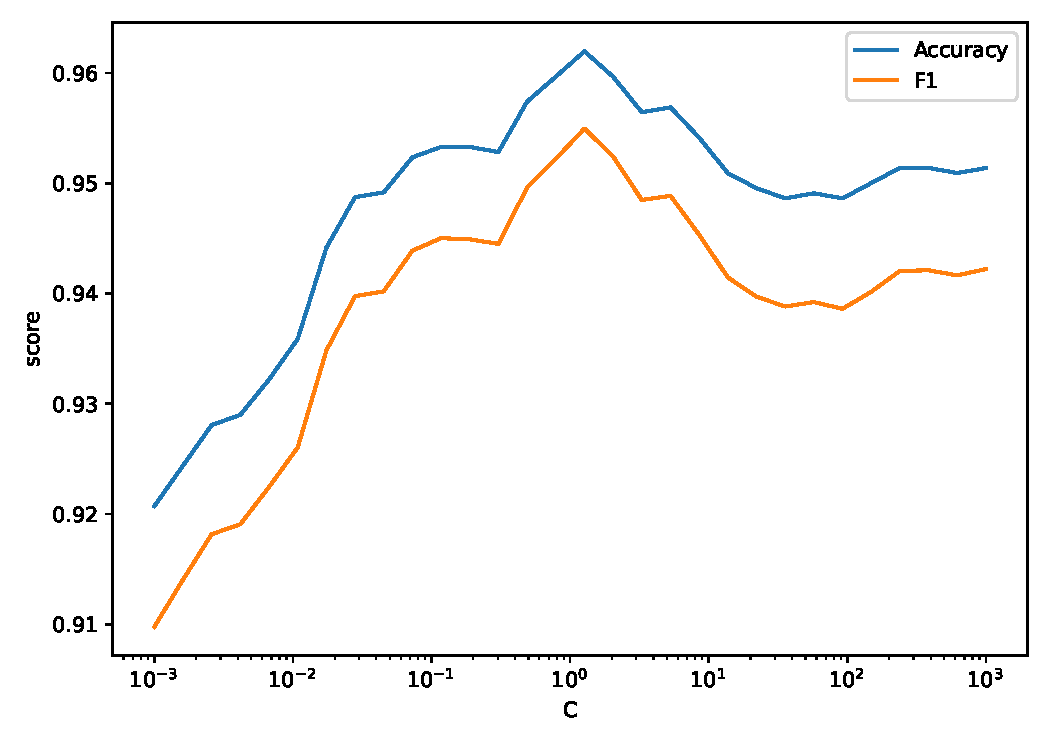
\includegraphics[width=\textwidth]{congress/plots/LinearSVC_C_sensitivity_new.pdf}
        \caption{Parameter \textsf{C} for dataset "Congressional Voting"}
    \end{subfigure}
    \hfill
    \begin{subfigure}[b]{0.45\textwidth}
        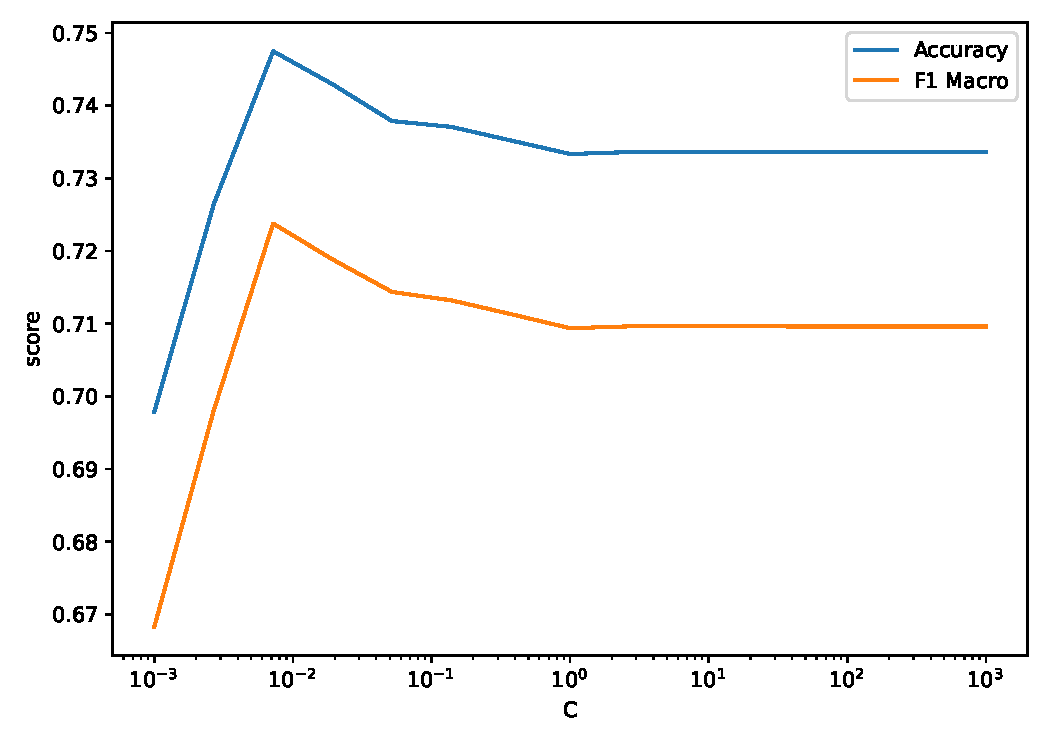
\includegraphics[width=\textwidth]{amazon/plots/LinearSVC_C_sensitivity.pdf}
        \caption{Parameter \textsf{C} for dataset "Amazon Commerce Reviews"}
    \end{subfigure}
    \caption{Sensitivity analysis of linear support vector classifier}
    \label{fig: sensitivity lsvc}
\end{figure}

We still have to analyze the sensitivity plots for the dataset "Diabetes" to figure out what parameter values are the best overall.\\
In figure \ref{fig:sensitivity svc diabetes} we can see, that for very small values of \textsf{C} the two scores diverge heavily, which means the \textsf{C} value found in table \ref{table:tu_hyp_svc_f1} is not suitable for optimizing accuracy and recall at the same time.\\
To get the best recall with still decent accuracy we choose \textsf{class\_weight}=\textsf{'balanced'} and \textsf{fit\_intercept}='True' and \textsf{C}=0.0452. This gives us an accuracy of 0.747 and a recall of 0.734.%20241113_110548 sensitivity analysis

\begin{figure}[h!]
    \centering
    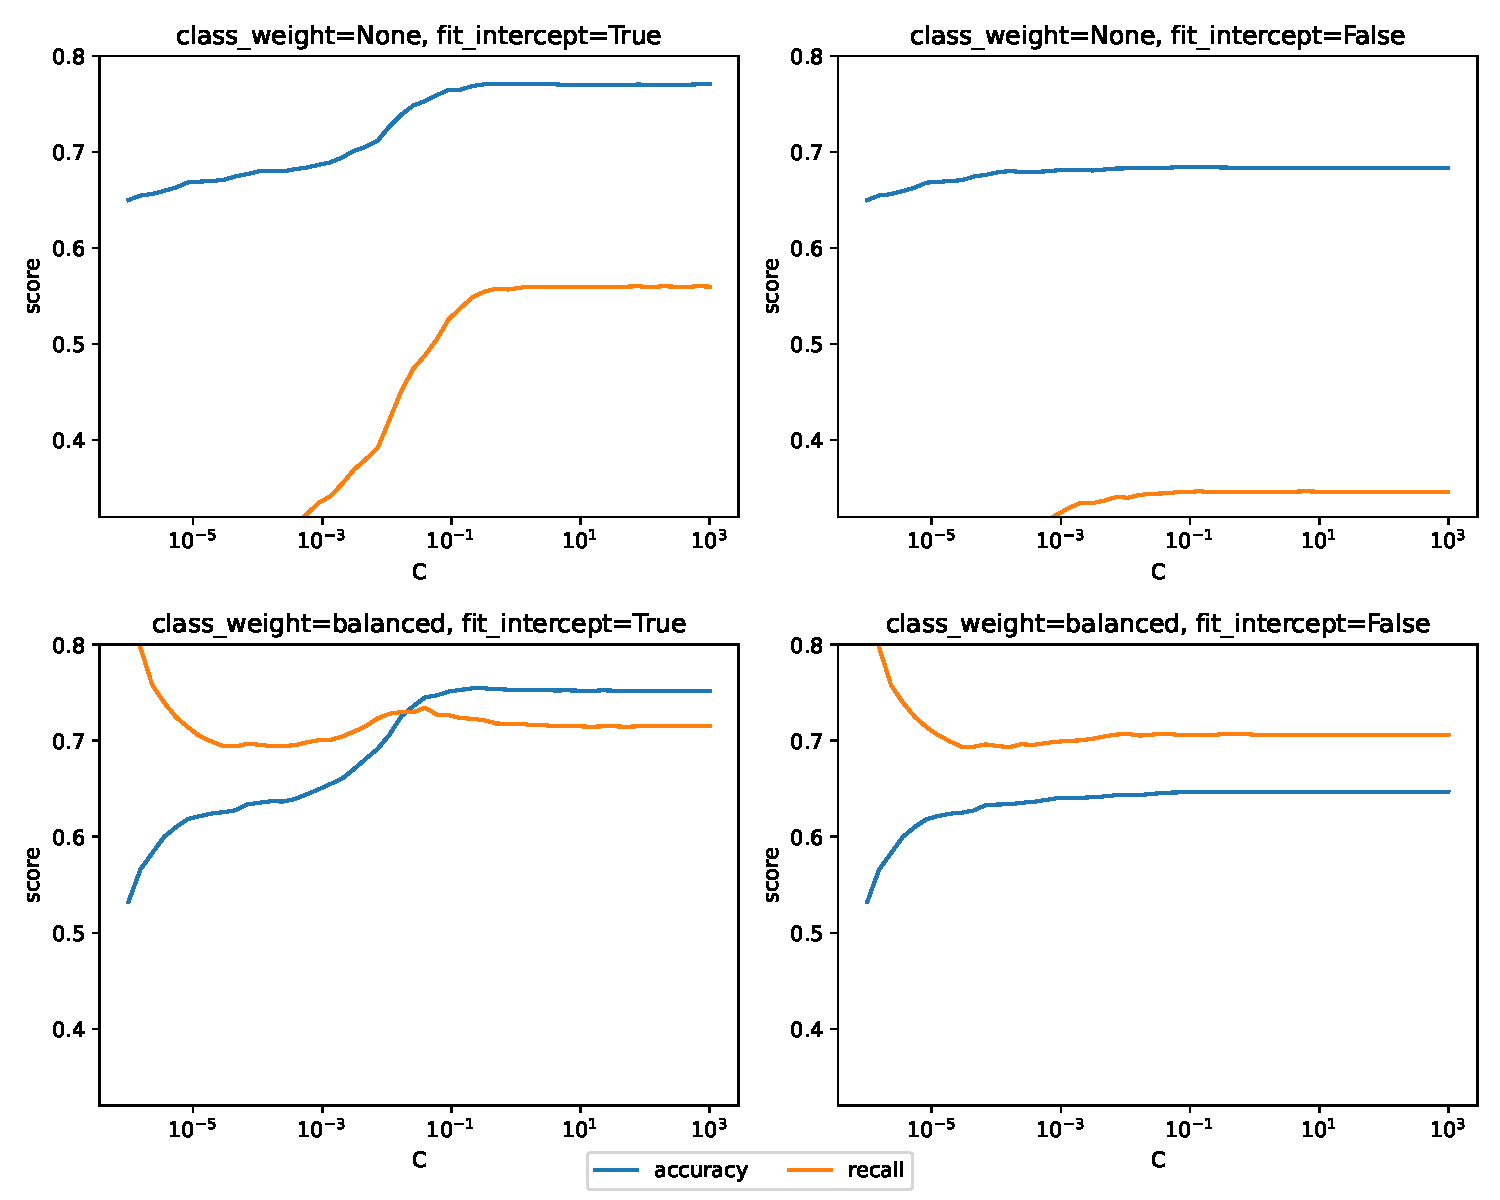
\includegraphics[width=\textwidth]{diabetes/plots/linearsvc_parameter_sensitivity.pdf}
    \caption{Sensitivity of Parameter \textsf{C} for datasets "Diabetes"}
    \label{fig:sensitivity svc diabetes}
\end{figure}

\textbf{Ridge Classifier Sensitivity:}

Interestingly we found that for the ridge classifier the parameter \textsf{alpha} hardly influenced the effectiveness scores of our models. While the measures were nearly left untouched by variation of \textsf{alpha} for the "Census Income" and the "Diabetes" dataset, the "Amazon Commerce Reviews" dataset showed a little variation  in accuracy and F1 score and the "Congressional Voting" showed a decrease in both metrics as one can see in figure \ref{fig: sensitivity ridge}, but the difference was not really significant considering the scaling of the plot.\\
Setting \textsf{class\_weight} to 'balanced' improved the F1 score/recall for the "Census Income" and the "Diabetes" dataset while lowering the accuracy as one could expect due to the bias variance trade off. For the other two datasets this hyperparameter did not really influence performance at all.\\
Finally, we want to analyze the parameter \textsf{fit\_intercept}. This parameter had no significant influence on the dataset "Census Income" and only slightly increased accuracy and F1 score when set to 'True' for "Congressional Voting". For "Amazon Commerce Reviews" interestingly setting it to 'False' increased the scores of both metrics by about .5 percentage points. The biggest influence that we could observe was when testing it on the "Diabetes" Dataset. Here \textsf{fit\_intercept}=False yielded a pretty significant increase in recall but a decrease in accuracy as one can see from figure \ref{fig:sensitivity ridge diabetes}.

\begin{figure}[h!]
    \captionsetup{justification=centering}
    \begin{subfigure}[b]{0.45\textwidth}
        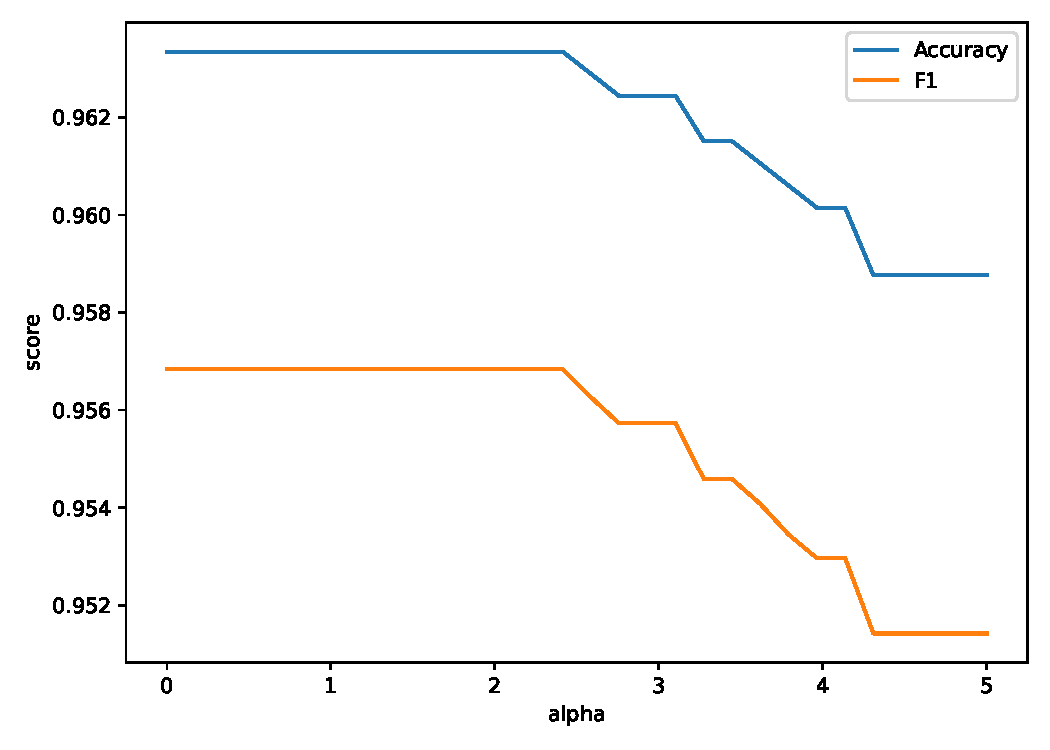
\includegraphics[width=\textwidth]{congress/plots/RidgeClassifier_alpha_sensitivity_new.pdf}
        \caption{Parameter \textsf{alpha} for dataset "Congressional Voting"}
    \end{subfigure}
    \hfill
    \begin{subfigure}[b]{0.45\textwidth}
        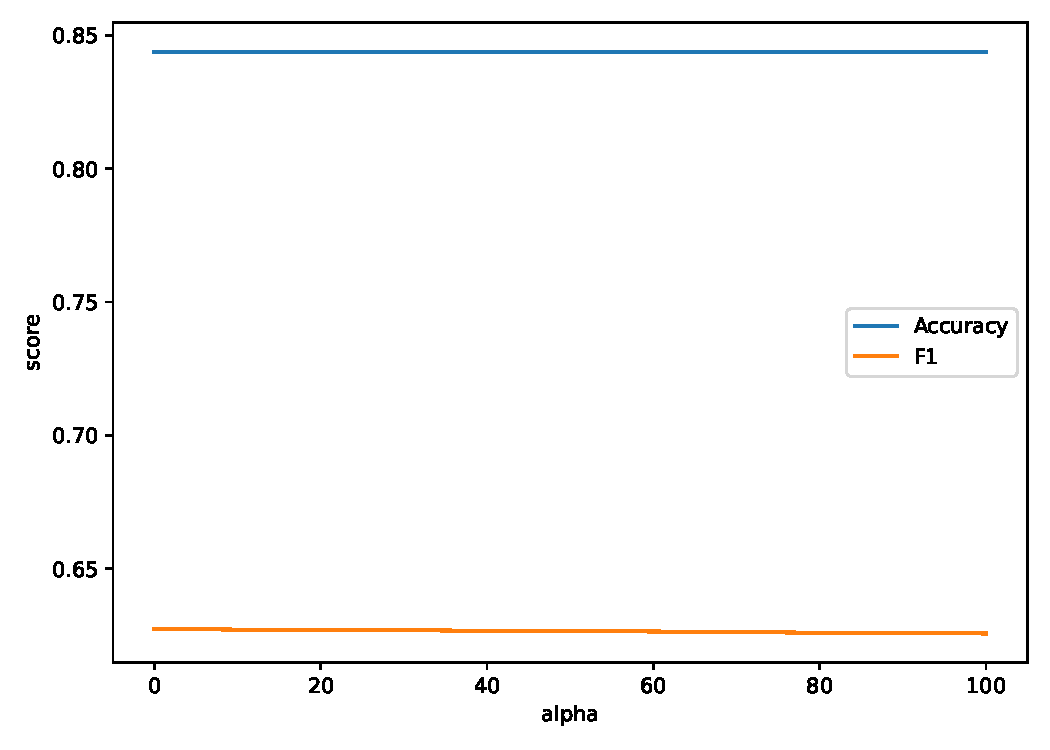
\includegraphics[width=\textwidth]{census/plots/RidgeClassifier_alpha_sensitivity.pdf}
        \caption{Parameter \textsf{alpha} for dataset "Census Income"}
    \end{subfigure}
    \caption{Sensitivity analysis of ridge classifier}
    \label{fig: sensitivity ridge}
\end{figure}

Once more we are not done yet, as we still need to decide on the best parameter setting for the "Diabetes" dataset.\\
We have already established, that changing \textsf{alpha} does not really influence the performance of the model, so the more important question is what combination of the other two parameters works best.\\
By looking at figure \ref{fig:sensitivity ridge diabetes} we can see that we have to set \textsf{class\_weight} to 'balanced' and \textsf{fit\_intercept} to 'False' when favoring recall over accuracy because this gives us the highest recall and in the other cases the recall was either a lot worse or the accuracy only increased marginally. For this combination of \textsf{fit\_intercept} and \textsf{class\_weight} the best value for alpha is 0 and we get an accuracy of 0.737 and a recall of 0.797.%20241113_115258 sensitivity analysis

\begin{figure}[h!]
    \centering
    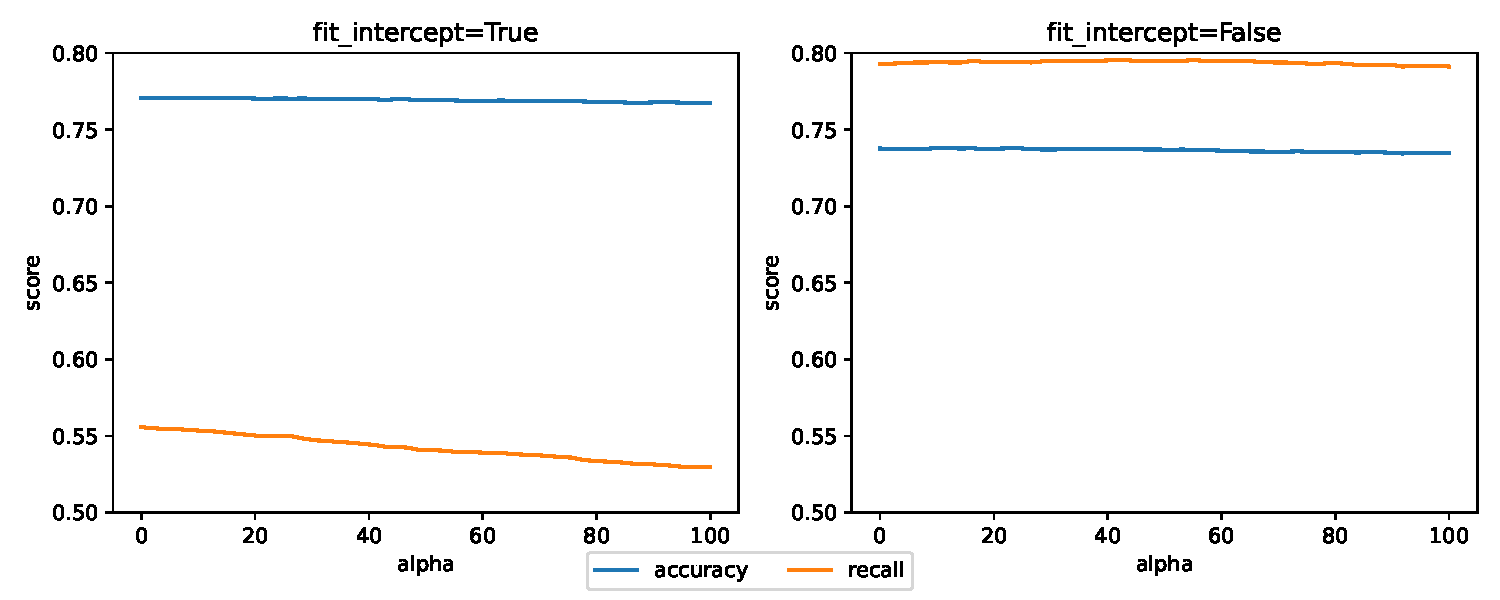
\includegraphics[width=\textwidth]{diabetes/plots/ridge_parameter_sensitivity.pdf}
    \caption{Sensitivity of Parameter alpha for datasets "Diabetes"}
    \label{fig:sensitivity ridge diabetes}
    \end{figure}



\section{Conclusion}
The goal of this section is to compare the classifiers for each dataset and give a general overview on the
performance of the tested classifiers. To make this comparison fair, we ensured to use exactly the same
splits within each dataset in the cross-validation. This is achieved by always using the same random state
when creating the splits. Of course we applied the most successful preprocessing steps as discussed in
section 4 and the hyperparameter settings established in section 5, which ensures that each classifier
performs as good as possible. This way we can accurately state which classification algorithm performed
best for each dataset.\\
In table~\ref{tab:best_results} we summarized the top performance measures for each dataset and classifier. We also compared
the best result for accuracy with the accuracy of the ”Dummy classifier”, which is shown in table 11.
The ”Dummy classifier” always predicts the majority class, so it can be used to establish a baseline. If
the accuracy of a classifier is better than this baseline, then that classifier must have learned something.
We can only use accuracy as a metric for the ”Dummy classifier”, because the F1 score is not defined as
you would divide by zero in the calculation.
\begin{table}[h!]
\centering
\footnotesize
\begin{tabular}{|l|c|c|c|c|c|c|c|c|}
\hline
& \multicolumn{2}{c|}{Congressional Voting} & \multicolumn{2}{c|}{Amazon Reviews} & \multicolumn{2}{c|}{Census Income} & \multicolumn{2}{c|}{Diabetes} \\
\hline
& Accuracy & F1 & Accuracy & F1 & Accuracy & F1 & Accuracy & Recall \\
\hline
Random Forest & 0.963 & 0.957 & 0.732 & 0.704 & 0.866 & 0.685 & 0.773 & 0.590 \\
\hline
LinearSVC & 0.963 & 0.956 & 0.748 & 0.725 & 0.853 & 0.659 & 0.747 & 0.734 \\
\hline
Ridge & 0.963 & 0.957 & 0.754 & 0.730 & 0.795 & 0.665 & 0.737 & 0.797 \\
\hline
Dummy & 0.613 & - & 0.020 & - & 0.759 & - & 0.653 & - \\
\hline
\end{tabular}
\vspace{0.3cm}
\caption{5-fold cross-validation results for each dataset and classifier}
\label{tab:best_results}
\end{table}

The scores in table~\ref{tab:best_results} are computed using repeated stratified 5-fold
cross-validation. We chose 10 repetitions for the datasets ”Congressional Voting” and ”Diabetes” and 5
repetitions for the other two datasets (due to runtime).
From this table we can conclude that on the datasets "Congressional Voting" and 
"Amazon Commerce Review" the ridge classifier
performed the best, although all classifiers performed almost the same. For the dataset "Census Income" we can see that
the random forest classifier is performing best with respect to both performance measures. Lastly,
for the "Diabetes" dataset the random forest classifier outperformed the others in both measures. But if we keep our preferences the same as in the
last few sections, we can conclude that either the linear support vector classifier or the ridge classifier
are the best choice for this dataset. \\
At this point we also want to compare cross-validation to the hold-out method. 
The hold-out method works by taking 70\% of the data as the training set and the remaining 30\% as the test set.
Then on the test set an evaluation is done. The cross-validation has already been introduced in a previous section.\\
The scores for the hold-out method
highly depend on the split and the model chosen as seen in figure~\ref{fig:model_comparison amazon},
where the box-plots are shown for the
"Amazon Commerce Review" dataset.



\begin{figure}[h!]
\centering
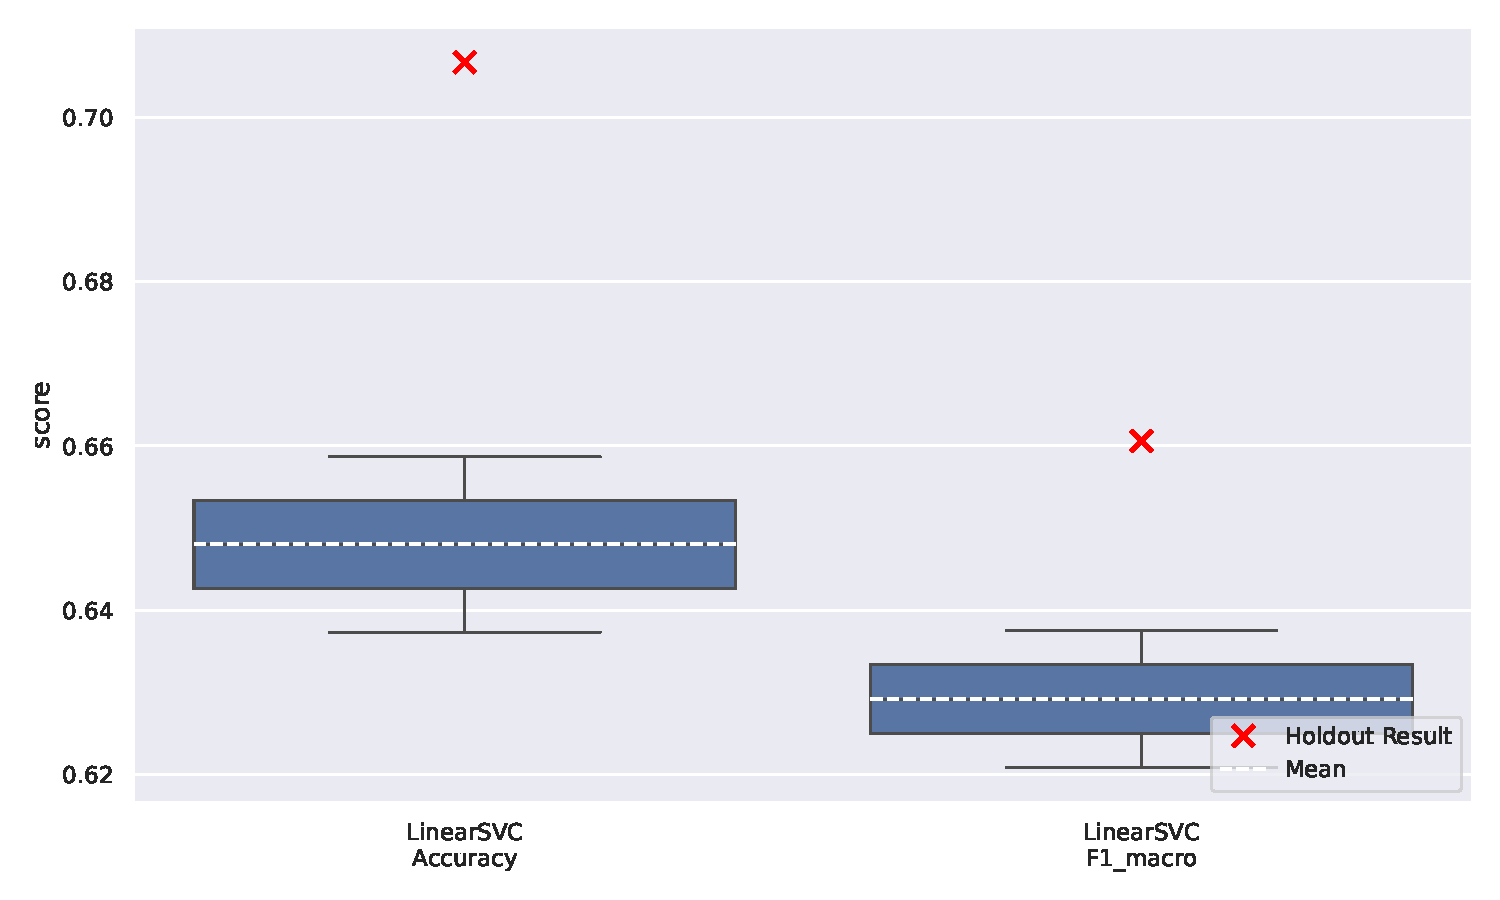
\includegraphics[width=\textwidth]{amazon/plots/model_comparison.pdf}
\caption{Model Comparison for "Amazon Commerce Review" dataset}
\label{fig:model_comparison amazon}
\end{figure}





 




We also want to compare the efficiency of the classifiers. For this we used the runtime of the hold-out
method calculation from above. We measured both the time for training (including preprocessing) and
the time it took the test the model. Those values are displayed in table~\ref{tab:runtime_models}.


\begin{table}[h!]
\centering
\footnotesize
\begin{tabular}{|c|c|c|c|c|c|c|c|c|}
\hline
\textbf{Model} & \multicolumn{2}{c|}{Census} & \multicolumn{2}{c|}{Amazon} & \multicolumn{2}{c|}{Congress} & \multicolumn{2}{c|}{Diabetes} \\
\hline
& \textbf{Train} & \textbf{Pred} & \textbf{Train} & \textbf{Pred} & \textbf{Train} & \textbf{Pred} & \textbf{Train} & \textbf{Pred} \\
\hline
LinearSVC & 0.17 & 0.02 & 0.51 & 0.02 & 0.00 & 0.00 & 0.00 & 0.00 \\
\hline
Ridge & 0.09 & 0.02 & 7.91 & 0.20 & 0.00 & 0.00 & 0.00 & 0.00 \\
\hline
RandomForest & 126.59 & 1.63 & 12.92 & 0.10 & 1.00 & 0.03 & 4.79 & 0.09 \\
\hline
\end{tabular}
\vspace{0.3cm}
\caption{Runtime of models for different datasets}
\label{tab:runtime_models}
\end{table}




On the contrary, the linear support vector classifier and ridge classifier performed similar
at the first glance. The results from "Amazon Commerce Review" and "Census Income" might suggest,
that the linear support vector classifier is faster for high dimensional datasets, whereas the ridge classifier
is quicker with a high number of instances. We found out that the parameter dual of the linear support
vector classifier has a great influence on its runtime. This parameter describes whether the algorithm
should solve for the primal or dual optimization problem. Let n be the number of samples and d the number
of dimensions of a dataset. The dual formulation requires the computation of an n × n matrix, whereas
in the primal formulation a d × d matrix is calculated. Therefore, the primal formulation is faster for
datasets, where n is greater than d, which was especially noticeable for the ”Census Income” dataset. Also, on the "Diabetes"
dataset as it is very low dimensional the dual procedure is faster. The results are shown in table~\ref{tab:dual_comparison}.

\begin{table}[h!]
\centering
\begin{tabular}{|c|c|c|}
\hline
\textbf{Dataset} & \textbf{Primal} & \textbf{Dual} \\
\hline
Census & 0.198 & 1.43 \\
\hline
Amazon & 2.27 & 0.648 \\
\hline
Census & 0.005 & 0.007 \\
\hline
Diabetes & 0.004 & 1.25 \\
\hline
\end{tabular}
\vspace{0.3cm}
\caption{Comparison of Dual and Normal Linear Support Vector classifier training time for different datasets}
\label{tab:dual_comparison}
\end{table}
After all experiments our final conclusion is that no classifier we used outperformed the other across all
datasets. The results in table \ref{tab:best_results} imply that the effectiveness of a classifier is highly dependent on the
dataset. What we can establish is that the linear support vector classifier was never the worst in both
metrics. Therefore, it seems to be a very versatile classifier. In comparison, n the success for random forests
varied quite a lot for different datasets and effectiveness measures. This could be due to the fact, that
decision trees generally tend to overfit the model. As for efficiency, table \ref{tab:runtime_models} highlighted a big weakness of
the random forest classifier, namely that it’s comparatively very slow. Summing up section \ref{sec:preprocessing}, choosing
the right preprocessing steps, especially the scaler and dimension reduction, influences the results notably,
though in varying magnitude for different classifiers and datasets. Here random forest seems to be the
least influenced by the choice of scaler as seen in tables \ref{table:censustransformers} and \ref{table:diabetesscalers}. The sensitivity analysis in section \ref{sec:hyperparameters}
showed how much of an impact even a single hyperparameter can have on the overall performance of a
model. However, comparing the results of section \ref{sec:preprocessing} with the ones in section \ref{sec:hyperparameters} and table \ref{tab:runtime_models}, it is clear that
tuning the parameters hardly influenced the result for the ”congressional voting” dataset. In contrast, the
recall score for the ”Diabetes” dataset and both effectiveness scores for the ”Amazon Commerce Reviews”
improved a lot after the parameter tuning. For the dataset ”Census Income” only the support vector
classifier improved after optimizing the F1 score. As a summary of this whole project we would say that
the best strategy for a classification problem majorly depends on the dataset in the beginning. Once a
classifier is chosen everything else depends on the combination of the two including the importance of
parameter tuning and preprocessing as well as the overall success.




\end{document}